% windsor's engineering notepad template
% uses emerald and lxfonts packages from ctan
%
% don't forget to change the date and other info in the header!!
%
% convert to bitmap with:
% convert -density 300x300 notes_template.pdf -resize 800x notes_template.png 

\documentclass[12pt]{article}
\usepackage[T1]{fontenc}
\usepackage{amsfonts}
\usepackage{emerald}
\usepackage{lxfonts}
\usepackage{amsmath}
\usepackage{graphicx}
\usepackage{eso-pic}
\usepackage{lastpage}
\usepackage[left=2.7cm,right=1.7cm,top=1.65cm,bottom=1.0cm]{geometry}

% configure page header
\usepackage{fancyhdr}
\setlength{\headheight}{15pt}
\pagestyle{fancy}\fancyhf{}
\renewcommand{\headrulewidth}{0pt}
\renewcommand{\footrulewidth}{0pt}
\lhead{\normalfont\ECFAugie \large{MATH 3E NOTES}}
\chead{\normalfont\ECFAugie \large{W. SCHMIDT}\hspace{1.4cm}}
\rhead{\normalfont\ECFAugie \large{\MakeUppercase{1/27/11}}\hspace{1.5cm}\thepage\hspace{0.1cm}/\hspace{0.1cm}\pageref{LastPage}\hspace{-1.5cm}}

% background image
\newcommand\BackgroundPic{
\put(0,0){
\parbox[b][\paperheight]{\paperwidth}{%
\vfill
\centering
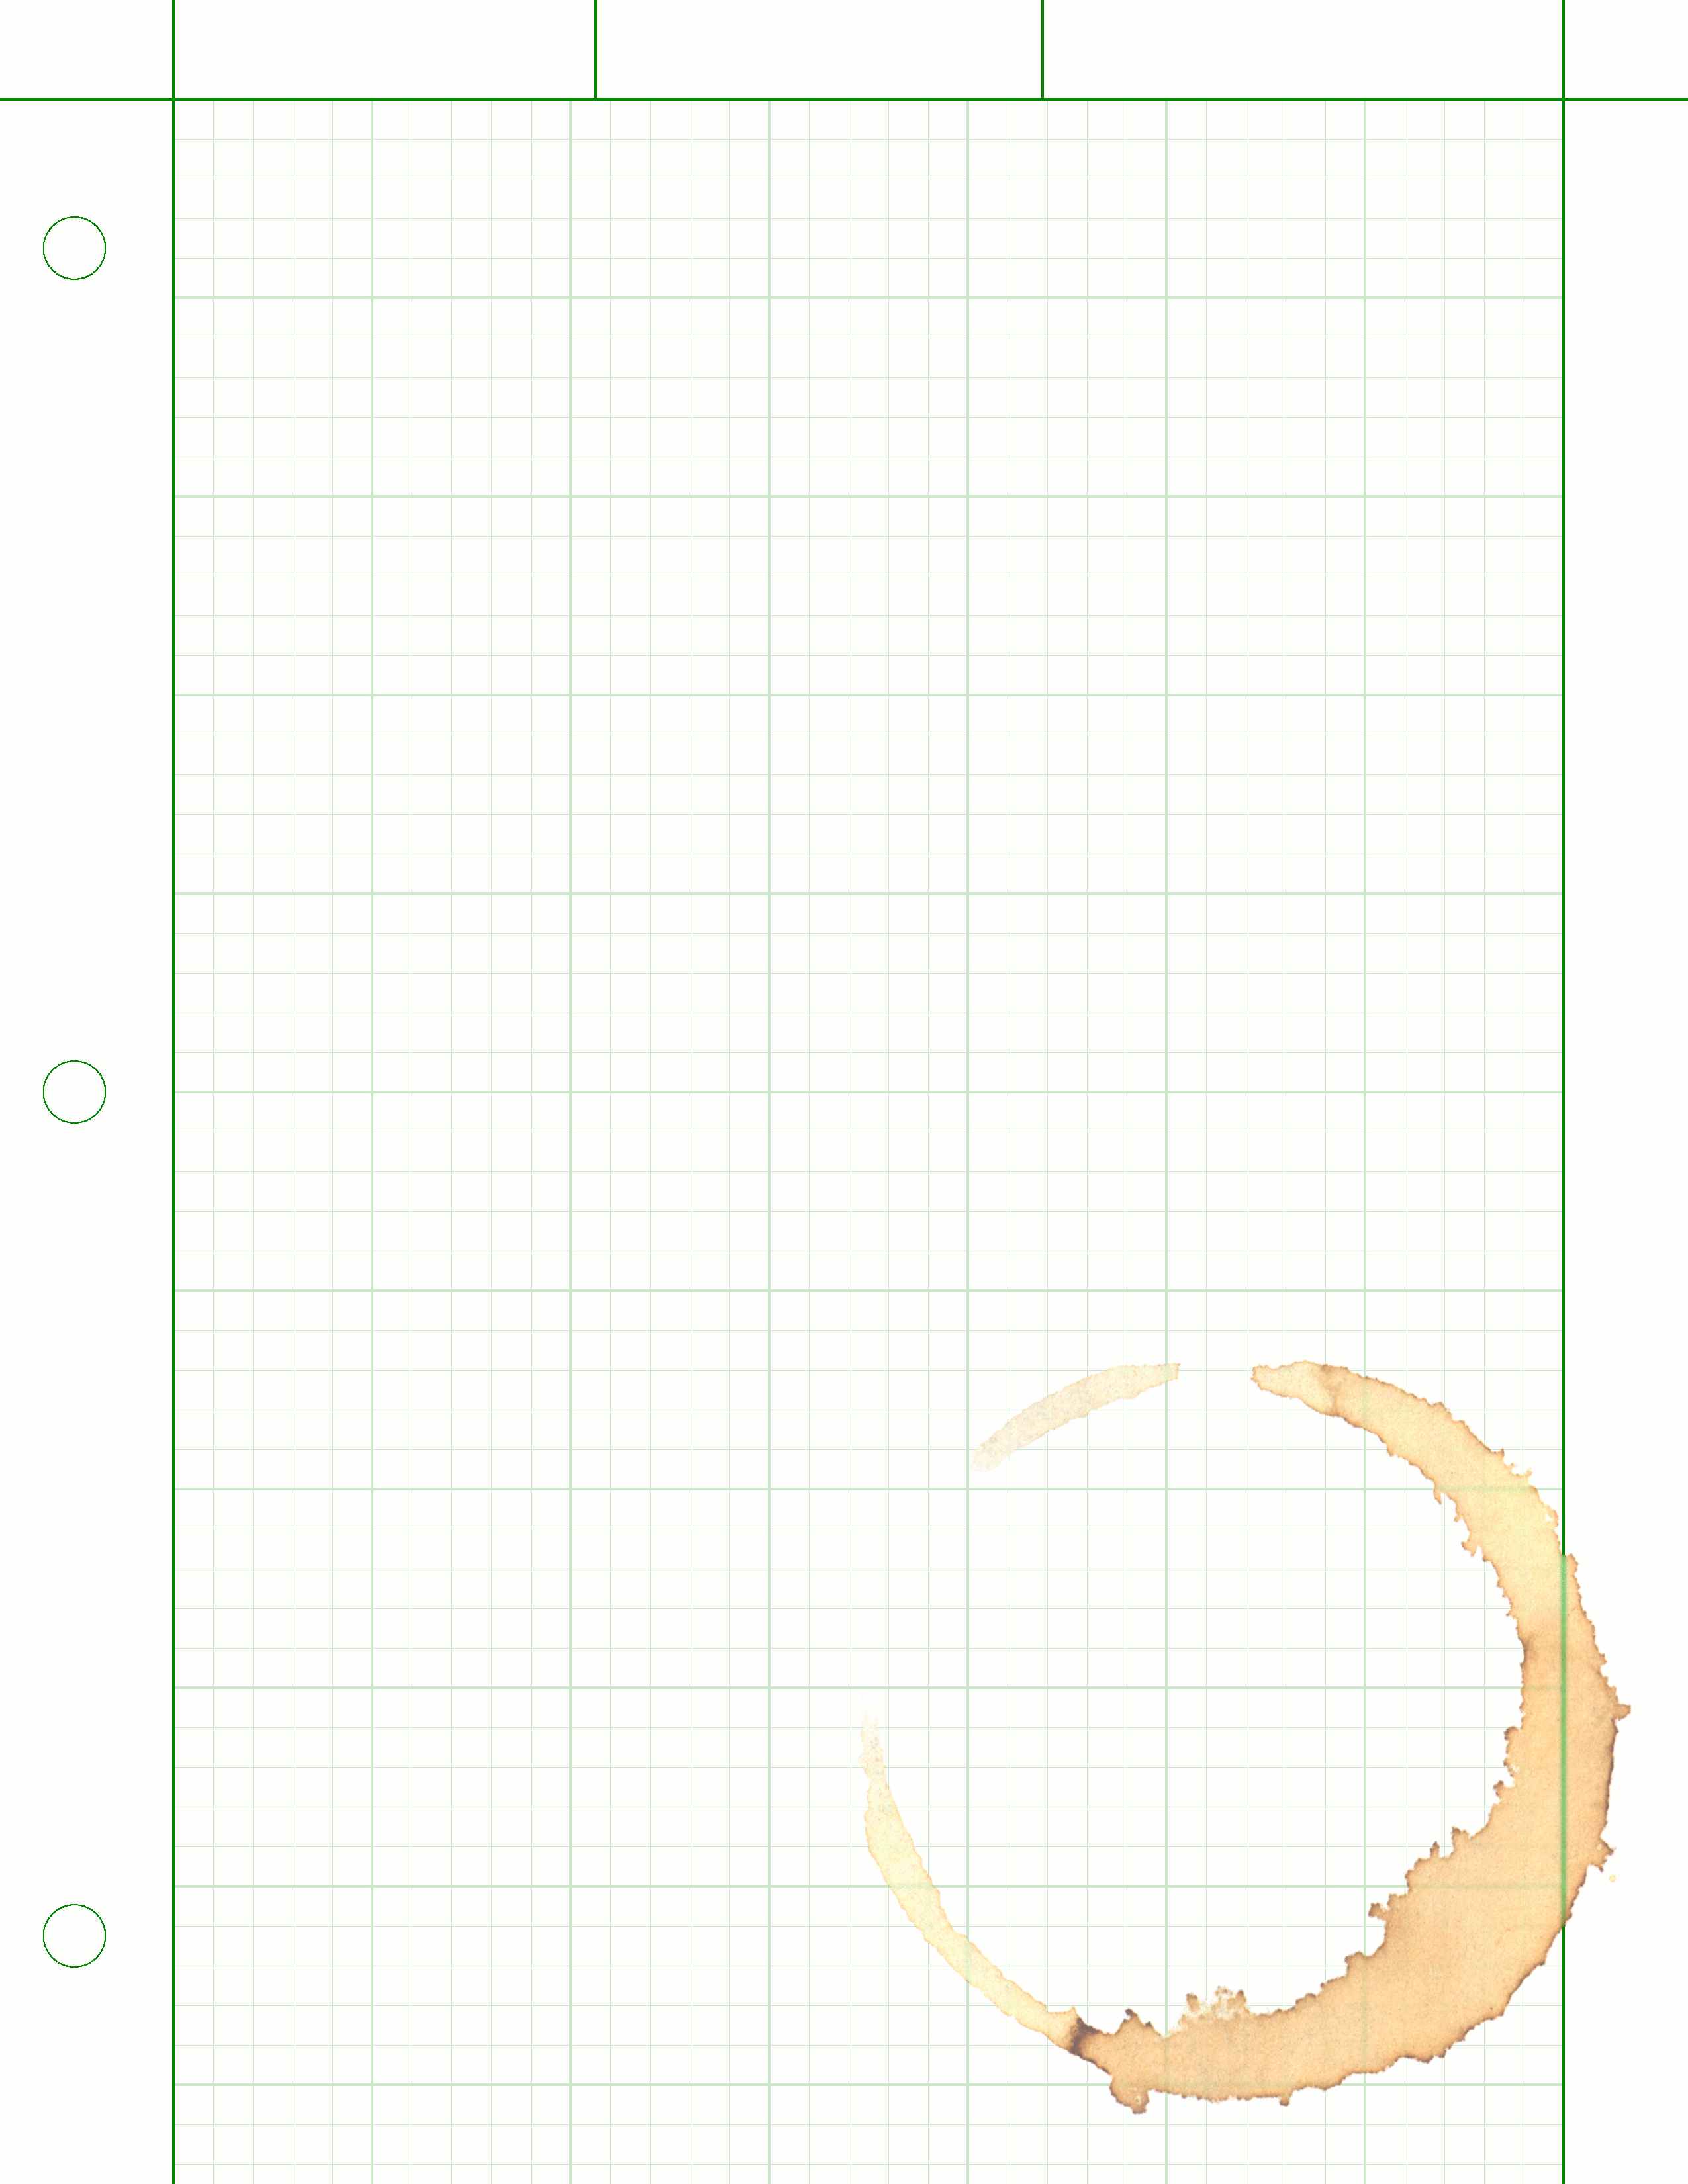
\includegraphics[width=\paperwidth,height=\paperheight,
keepaspectratio]{background.png}%
\vfill
}}}

% configure section titles
\usepackage{titlesec}
\titleformat{\section}{\Large}{\thesection}{1em}{}
\titleformat{\subsection}{\large\bfseries}{\thesubsection}{1em}{}

\begin{document}
\AddToShipoutPicture{\BackgroundPic}
\normalfont\ECFAugie

% custom commands
\newcommand{\windef}[1]{\subsection*{\underline{DEF:} \normalsize{#1}}} % definition
\newcommand{\winex}[1]{\subsection*{\underline{EX:} \normalsize{#1}}} % example
\newcommand{\winsec}[1]{\section*{\underline{#1}}} % section
\newcommand{\winres}[1]{\begin{math}\Rightarrow\left\{\begin{matrix}#1\end{matrix}\right.\end{math}\hspace{0.2cm}} % result
\newcommand{\winsys}[1]{\begin{math}\left\{\begin{matrix}#1\end{matrix}\right.\end{math}} % system
\newcommand{\winero}[1]{\begin{math}\xrightarrow{#1}\end{math}} % row operation
\newcommand{\winmat}[1]{\begin{math}\begin{bmatrix}#1\end{bmatrix}\end{math}} % matrix
\newcommand{\winsub}[1]{\subsection*{$\star$\hspace{0.2cm} #1}} % dot
\newcommand{\step}[1]{\begin{math}\xrightarrow{\text{#1}}\end{math}} % step in a process
\newcommand{\winrtwo}{\begin{math}\text{R}^\text{2}\end{math}}
\newcommand{\winrthree}{\begin{math}\text{R}^\text{3}\end{math}}
\newcommand{\wineq}[1]{\begin{equation}\notag#1\end{equation}}

%%%%%%%%%%%%%%%%%%%%%%
% start writing here %
%%%%%%%%%%%%%%%%%%%%%%

% section
\winsec{section name goes here}

% term definition
\winsub{term definition}
\windef{term - and it's definition}

% example
\winsub{an example}
\winex{example heading}

% system of equations
\winsub{a system of equations}
\winsys{
2x+4y=2 \\
2x+6y=3}

% matrix
\winsub{working a multistep problem}
\winmat{
a & b & c \\
d & e & f \\
g & h & i }
% row operation
\winero{R_1+R_2}
% matrix
\winmat{
a & b & c \\
d & e & f \\
g & h & i }
% result
\winres{
x = 1 \\
y = 2 \\
z = 3}

% vector in 3-space
\winsub{a vector in \winrthree}
v = \winmat{
x \\
y \\
z }

\winsub{a multi-step process}
A \step{do stuff} B \step{more stuff} C

% numbered list
\winsub{an enumerated list}
\begin{enumerate}
\item{this is the first item in an enumerated list}
\item{this is the second item in an enumerated list}
\end{enumerate}

% manual line breaks
\winsub{manually broken lines}
the first line\\
the second line\\
the third line

% equation
\winsub{some math}
\wineq{
\int_a^b \! f(x) \; dx % definite
\int \! f(x) \, dx \; % indefinite
\frac{\pi}{2} \; % fraction
\sqrt{\theta} \; % root
n = 1,2,3 \ldots 4}

\end{document}
